\chapter{Nyttevirkningsmåling på effektforstærker}
\label{maalejournal-nytte}

Denne målerapport dokumenterer målinger foretaget på projektets effektforstærker, opbygget som beskrevet i kapitel \ref{effektforstaerker}. Målingerne er foretaget på Fredrik Bajers Vej 7 i lokale B1-104 på Aalborg Universitet den 17. december 2010 af gruppe 311.

\subsection*{Formål}

Målingernes formål er at teste effektforstærkerens nyttevirkning.


\subsection*{Testobjekt}
Der testes i disse målinger på effektforstærkeren, som beskrevet i kapitel \ref{effektforstaerker}. På figur \ref{fig:testob_efforstaerker_nytte} er denne vist, med angivelse af terminalerne anvendt i målingen.

\begin{figure}[h]
\centering
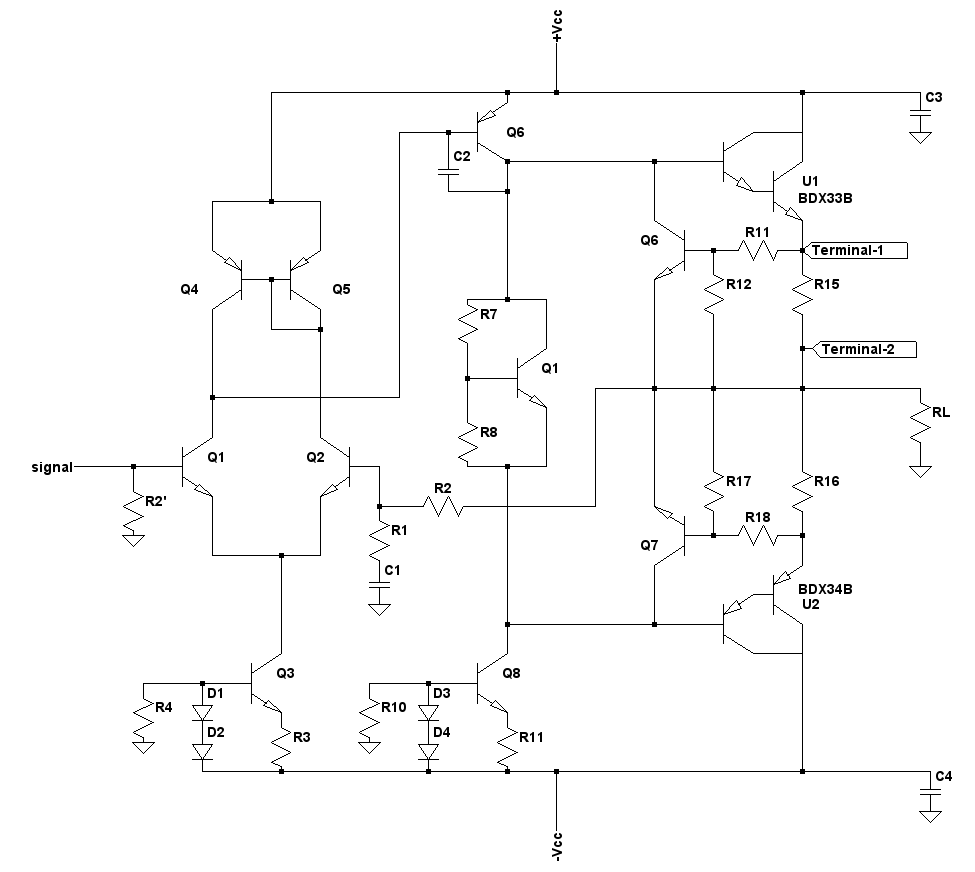
\includegraphics[width=\textwidth]{maalerapporter/effektforstaerker/effektforstaerker_nyttevirkning_test.png}
\caption{Effektforstærker med angivelser af de anvendte terminaler}
\label{fig:testob_efforstaerker_nytte}
\end{figure}

\subsection*{Måleopstilling}
Målingerne foretages  ved en opstilling, der måler spændingsfaldet over $R_{15}$ og $R_L$ for at kunne bestemme nyttevirkningen. Opstillingerne er vist på figur \ref{fig:maaleop-nytte}.

\begin{figure}[h]
\centering
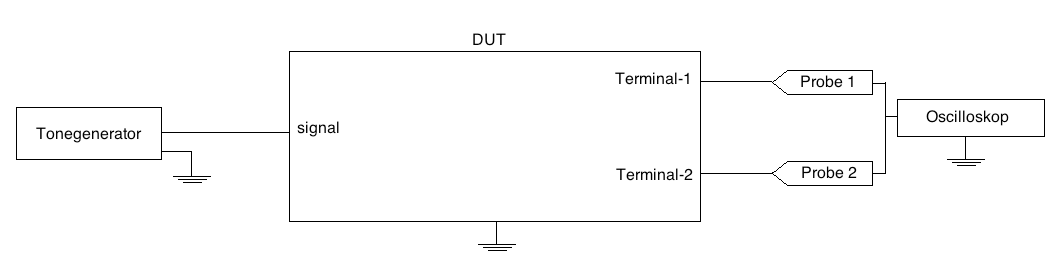
\includegraphics[scale=0.3]{maalerapporter/effektforstaerker/opstilling_nyttevirkning.png}
\caption{Måleopstilling for måling af nyttevirkning i effektforstærkeren}
\label{fig:maaleop-nytte}
\end{figure}

\subsection*{Teori}
For at finde nyttevirkningen for effektforstærkeren skal den samlede effekt afsat i effektforstærkeren samt effekten afsat i $R_L$ findes. Dette skyldes at nyttevirkningen er givet ved formel \ref{eq:nyttevirkning_beregning}.

\begin{equation}
\eta = \frac{P_{R_L}}{P_\mathrm{samlet}}
\label{eq:nyttevirkning_beregning}
\end{equation}

For at finde den samlede effekt måles spændingsfaldet over $R_{15}$ for at finde den strøm der løber. Denne strøm anses for at være den samlede strøm tilført effektforstærkeren. Der ses bort fra strømmen som løber i differensforstærkeren og spændingsforstærkeren grundet deres lille størrelse. Strømmen gennem $R_{15}$ beregnes med Ohms lov og effekten afsat i hele effektforstærkeren beregnes med formel \ref{eq:effekt_beregning}.

\begin{equation}
P=V \cdot I_\mathrm{rms}
\label{eq:effekt_beregning}
\end{equation}

Den samme måling og beregning udføres for $R_L$ for derefter at beregne nyttevirkningen med formel \ref{eq:nyttevirkning_beregning}.

\subsection*{Anvendt udstyr}
\begin{table}[h]
\centering
\begin{tabular}{l|c|l}
\hline\hline
Instrument & AAU-nr. & Fabrikant, type m.v. \\
\hline\hline
Oscilloskop & 33843 & Agilent 54621A \\[4pt]
Oscillator & 07995 & B\&O RC-oscillator TG7 \\[4pt]
Spændingsforsyning & 33896 & HAMEG HM7042 \\[4pt]
Effektmodstand 8,2~\ohm & 215901 & Ikke Angivet \\[4pt]
\hline\hline
\end{tabular}
\label{tab:maaleudstyr_effektforstaerker_nytte}
\end{table}
\clearpage
\subsection*{Måleprocedure}
Proceduren for at måle nyttevirkning er som følger:

\begin{enumerate}
\item Spændingsforsyningen indstilles $\pm$23 V og tilsluttes
\item Testobjektet tilsluttes som på figur \ref{fig:maaleop-nytte}
\item Oscillatoren indstilles til 2 V peakspænding og 1 kHz
\item Spændingsfaldet over $R_L$ og $R_{15}$ noteres
\end{enumerate}

\subsection*{Resultater}

Peakspændingen over $R_{15}$ blev målt til 1,5 V og over $R_L$ til 17,5 V. Dermed kan nyttevirkningen beregnes ud fra formlerne i teoriafsnittet.

\[ I_{R_{15}}=\frac{\frac{1,5~\mathrm{V}}{\sqrt{2}}}{0,68~\ohm}=1,56~\mathrm{A} \]
\[ P_\mathrm{samlet} = 23~\mathrm{V} \cdot 1,56~\mathrm{A}=35,9~\mathrm{W} \]
\[ I_{R_L}= \frac{\frac{17,5~\mathrm{V}}{\sqrt{2}}}{8,2~\ohm}=1,51~\mathrm{A} \]
\[ P_{R_L} = 17,5~\mathrm{V} \cdot 1,51~\mathrm{A}=18,7~\mathrm{W} \]
\[ \eta = \frac{18,7~\mathrm{W}}{35,9~\mathrm{W}}=53,4~\% \]

